% IEEE conference paper skeleton (3-6 pages). Compile on Overleaf: upload this file + the
% report/tables and results/figures folders (or fix the paths below).
% IMPORTANT: replace every [TODO] with YOUR OWN words. The rubric penalises unedited AI text.
\documentclass[conference]{IEEEtran}
\usepackage{booktabs, graphicx, cite, amsmath}
\graphicspath{{../results/figures/}}

\begin{document}
\title{Insurance Claim Fraud Detection Using Machine Learning with Nested Cross-Validation}
\author{\IEEEauthorblockN{Bhoomi Tiple}
\IEEEauthorblockA{Department of Software Engineering\\MIT Academy of Engineering, Alandi (D), Pune, India}}
\maketitle

\begin{abstract}
% 150-250 words: [problem] -> [objective] -> [method] -> [main numeric result].
[TODO]
\end{abstract}
\begin{IEEEkeywords}
insurance fraud, machine learning, class imbalance, nested cross-validation, explainability
\end{IEEEkeywords}

\section{Introduction}
% Why insurance fraud matters; why it is hard (few fraud cases); your objective; your contributions (list 2-3).
[TODO]

\section{Related Work}
% Review 10-15 papers from the last 5 years. Group them (e.g. classical ML, ensemble/boosting,
% imbalance handling, deep learning). End with the RESEARCH GAP and what you contribute.
[TODO] \cite{ref1}

% Literature table (one row per paper):
% Ref | Year | Dataset | Method | Key result | Limitation

\section{Methodology}
\subsection{Dataset}
% Source, number of claims, number of features, fraud percentage (see results/tables/eda_summary.csv,
% split_summary.csv and figure 01_class_balance).
[TODO]
\subsection{Preprocessing and Pipeline}
% Dropped ID columns, '?' treated as missing, engineered features (policy age, month, weekday,
% claim-to-premium ratio), median / 'Missing' imputation, scaling, one-hot encoding -- all inside a Pipeline.
[TODO]
\subsection{Models, Imbalance Handling and Validation}
% Dummy baseline, Logistic Regression, Random Forest, Gradient Boosting, SVM; class weighting;
% stratified 80/20 split (seed 42); 5x3 repeated stratified CV; GridSearchCV inside 5x3 nested CV;
% test set used once. Insert a block diagram of the pipeline here.
[TODO]

\section{Results and Discussion}
\subsection{Model comparison}
\begin{table}[t]\centering\caption{Repeated stratified CV results (mean $\pm$ std).}\label{tab:base}
\resizebox{\columnwidth}{!}{\begin{tabular}{lllllll}
\toprule
Model & Accuracy & Precision & Recall & F1 & ROC-AUC & PR-AUC \\
\midrule
Dummy (baseline) & 0.620 $\pm$ 0.044 & 0.242 $\pm$ 0.087 & 0.251 $\pm$ 0.089 & 0.246 $\pm$ 0.088 & 0.496 $\pm$ 0.059 & 0.254 $\pm$ 0.031 \\
Logistic Regression & 0.819 $\pm$ 0.026 & 0.610 $\pm$ 0.051 & 0.769 $\pm$ 0.055 & 0.678 $\pm$ 0.040 & 0.867 $\pm$ 0.021 & 0.675 $\pm$ 0.055 \\
Random Forest & 0.815 $\pm$ 0.026 & 0.617 $\pm$ 0.053 & 0.680 $\pm$ 0.055 & 0.646 $\pm$ 0.046 & 0.847 $\pm$ 0.028 & 0.589 $\pm$ 0.042 \\
Gradient Boosting & 0.829 $\pm$ 0.026 & 0.641 $\pm$ 0.050 & 0.710 $\pm$ 0.080 & 0.672 $\pm$ 0.054 & 0.859 $\pm$ 0.035 & 0.631 $\pm$ 0.066 \\
SVM (RBF) & 0.802 $\pm$ 0.025 & 0.594 $\pm$ 0.053 & 0.658 $\pm$ 0.046 & 0.623 $\pm$ 0.037 & 0.813 $\pm$ 0.026 & 0.564 $\pm$ 0.046 \\
\bottomrule
\end{tabular}
}\end{table}
\begin{table}[t]\centering\caption{Nested CV results after tuning.}\label{tab:nested}
\resizebox{\columnwidth}{!}{\begin{tabular}{lllllll}
\toprule
Model & Accuracy & Precision & Recall & F1 & ROC-AUC & PR-AUC \\
\midrule
Logistic Regression & 0.819 $\pm$ 0.029 & 0.608 $\pm$ 0.056 & 0.783 $\pm$ 0.041 & 0.683 $\pm$ 0.038 & 0.862 $\pm$ 0.020 & 0.662 $\pm$ 0.073 \\
Random Forest & 0.828 $\pm$ 0.028 & 0.628 $\pm$ 0.055 & 0.763 $\pm$ 0.045 & 0.687 $\pm$ 0.044 & 0.841 $\pm$ 0.029 & 0.600 $\pm$ 0.046 \\
Gradient Boosting & 0.856 $\pm$ 0.023 & 0.657 $\pm$ 0.046 & 0.894 $\pm$ 0.043 & 0.756 $\pm$ 0.032 & 0.864 $\pm$ 0.032 & 0.683 $\pm$ 0.064 \\
SVM (RBF) & 0.810 $\pm$ 0.033 & 0.602 $\pm$ 0.062 & 0.707 $\pm$ 0.072 & 0.648 $\pm$ 0.057 & 0.824 $\pm$ 0.026 & 0.594 $\pm$ 0.060 \\
\bottomrule
\end{tabular}
}\end{table}
\subsection{Ablation study}
\begin{table}[t]\centering\caption{Ablation: effect of removing one component.}\label{tab:abl}
\resizebox{\columnwidth}{!}{\begin{tabular}{lllll}
\toprule
Variant & F1 & Recall & PR-AUC & Δ F1 vs full \\
\midrule
Full model & 0.755 $\pm$ 0.028 & 0.894 $\pm$ 0.041 & 0.681 $\pm$ 0.056 & +0.000 \\
- class weighting (no balancing) & 0.673 $\pm$ 0.050 & 0.708 $\pm$ 0.084 & 0.689 $\pm$ 0.055 & -0.082 \\
- feature scaling & 0.755 $\pm$ 0.028 & 0.894 $\pm$ 0.041 & 0.681 $\pm$ 0.056 & +0.000 \\
- engineered features & 0.754 $\pm$ 0.027 & 0.891 $\pm$ 0.036 & 0.681 $\pm$ 0.057 & -0.002 \\
- claim amounts & 0.754 $\pm$ 0.027 & 0.892 $\pm$ 0.038 & 0.687 $\pm$ 0.051 & -0.001 \\
- insured hobbies & 0.622 $\pm$ 0.037 & 0.658 $\pm$ 0.044 & 0.496 $\pm$ 0.055 & -0.134 \\
- incident severity & 0.456 $\pm$ 0.049 & 0.515 $\pm$ 0.070 & 0.529 $\pm$ 0.050 & -0.299 \\
- demographics & 0.754 $\pm$ 0.027 & 0.892 $\pm$ 0.041 & 0.676 $\pm$ 0.058 & -0.001 \\
class weighting -> SMOTE & 0.734 $\pm$ 0.040 & 0.845 $\pm$ 0.060 & 0.683 $\pm$ 0.053 & -0.021 \\
\bottomrule
\end{tabular}
}\end{table}
\subsection{Test-set performance and error analysis}
\begin{table}[t]\centering\caption{Final held-out test metrics.}\label{tab:test}
\resizebox{\columnwidth}{!}{\begin{tabular}{lrrrrrrr}
\toprule
model & accuracy & precision & recall & f1 & roc\_auc & pr\_auc & mcc \\
\midrule
Gradient Boosting & 0.845000 & 0.636000 & 0.857000 & 0.730000 & 0.828000 & 0.617000 & 0.639000 \\
\bottomrule
\end{tabular}
}\end{table}
\begin{figure}[t]\centering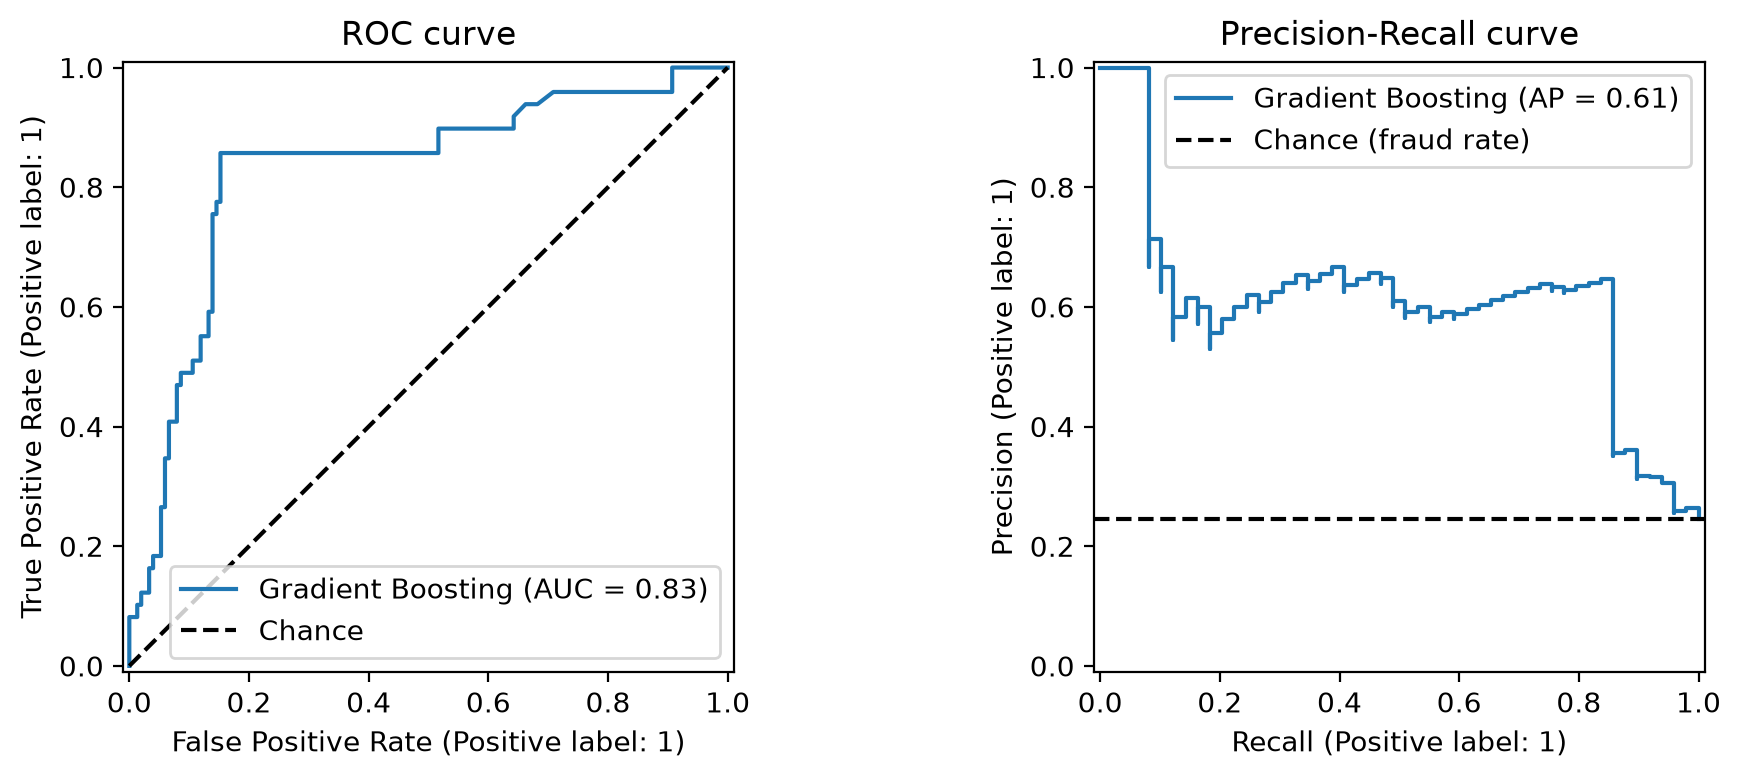
\includegraphics[width=\columnwidth]{09_roc_pr_curves.png}
\caption{ROC and precision-recall curves on the test set.}\end{figure}
\begin{figure}[t]\centering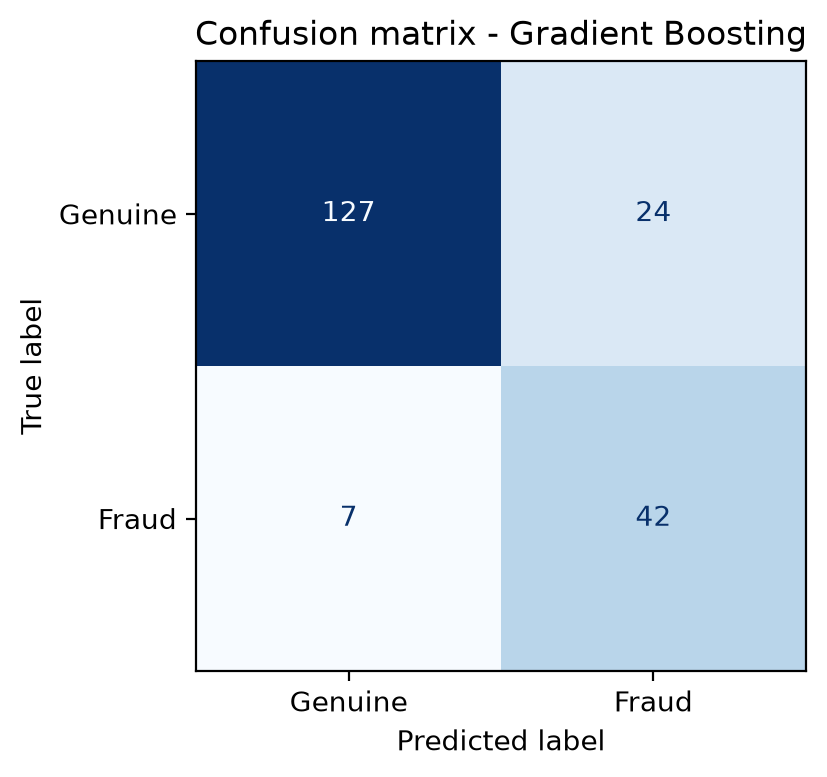
\includegraphics[width=0.7\columnwidth]{08_confusion_matrix.png}
\caption{Confusion matrix on the test set.}\end{figure}
\begin{figure}[t]\centering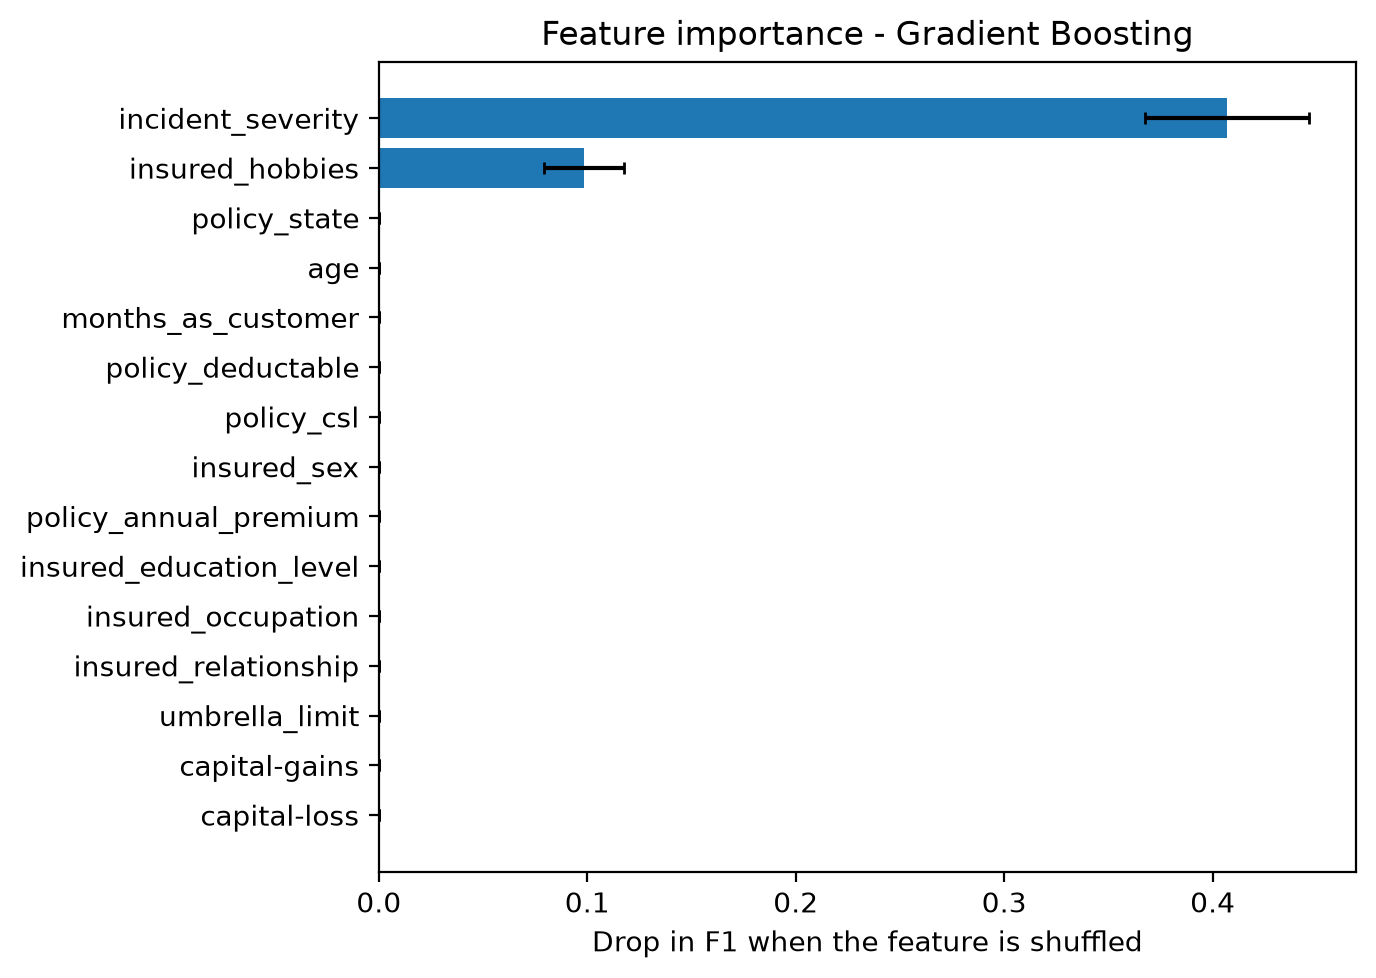
\includegraphics[width=\columnwidth]{10_feature_importance.png}
\caption{Permutation feature importance.}\end{figure}
% Discuss: which model won and why; what the ablation shows; which frauds were missed; honest limitations
% (small dataset, one source, public data, no cost-sensitive analysis, threshold fixed at 0.5).
[TODO]

\section{Conclusion and Future Work}
[TODO]

\begin{thebibliography}{00}
% 15-25 IEEE-style references, each cited in the text. Example format:
\bibitem{ref1} A. Author, B. Author, ``Title of paper,'' \textit{Journal Name}, vol. X, no. Y, pp. 1--10, 2023.
\end{thebibliography}
\end{document}
